\section{Appendix for chapter 2}

\subsection{Computation of diagonal elements of weight matrix}
\label{a.1}
Diagonal elements of weight matrix $\bm{W}$, the Hessian of log of Cox'x partial likelihood function, has the form 
\begin{displaymath}
w_i=\sum_{k\in C_i}\frac{d_k e^{\tilde{\eta}_i}}{\sum_{j\in R_i}e^{\tilde{\eta}_j}}-\sum_{k\in C_i}\frac{d_k (e^{\tilde{\eta}_i})^2}{(\sum_{j\in R_i}e^{\tilde{\eta}_j})^2}. 
\end{displaymath}
The two sums $\sum_{k\in C_i}$ and $\sum_{j\in R_i}$ both have $n$ elements, hence it is a $O(n^2)$ computation. However, if we notice the difference between $R_k$ and $R_{k+1}$ is the observations that are in $R_k$ but not in $R_{k+1}$, i.e., $\{j:t_k\leq y_j < t_{k+1}\}$, provided that the observed times $\bm{y}$ are sorted in non-decreasing order, then $\sum_{j\in R_k}e^{\tilde{\eta}_j}$ can be calculated as cumulative sums:
\begin{displaymath}
\sum_{j\in R_k} e^{\tilde{\eta}_j} =\sum_{j\in R_{k+1}} e^{\tilde{\eta}_j}+ \sum_{j\in R_k \& j\notin R_{k+1}} e^{\tilde{\eta}_j}.
\end{displaymath}
The same cumulative sum idea can be applied to $\sum_{k\in C_i}$: 
\begin{align*}
    \sum_{k\in C_{i+1}}\frac{d_k e^{\tilde{\eta}_i}}{\sum_{j\in R_i}e^{\tilde{\eta}_j}}&=\sum_{k\in C_i}\frac{d_k e^{\tilde{\eta}_i}}{\sum_{j\in R_i}e^{\tilde{\eta}_j}}+\sum_{k\in C_i\&k\notin c_{i+1}}\frac{d_k e^{\tilde{\eta}_i}}{\sum_{j\in R_i}e^{\tilde{\eta}_j}}, \\
    \sum_{k\in C_{i+1}}\frac{d_k (e^{\tilde{\eta}_i})^2}{(\sum_{j\in R_i}e^{\tilde{\eta}_j})^2}&=\sum_{k\in C_i}\frac{d_k (e^{\tilde{\eta}_i})^2}{(\sum_{j\in R_i}e^{\tilde{\eta}_j})^2}+ \sum_{k\in C_i\&k\notin c_{i+1}}\frac{d_k (e^{\tilde{\eta}_i})^2}{(\sum_{j\in R_i}e^{\tilde{\eta}_j})^2}.
\end{align*}
The equations above only calculate the sums once, and add at each sample index, which brings the computation cost down to linear time, $O(n)$. Considering sorting observed times as a data pre-processing procedure, the overall computation time for the weights is $O(n\log n)$.

\subsection{Solve regularized weighted least squares with cyclic coordinate descent}
\label{a.2}
To solve regularized weighted least squares, equation \eqref{eq2.9}, we first compute the gradient at current estimates of $(\tilde{\bm{\gamma}}, \tilde{\bm{\alpha}})$. Let $\gamma_j$ be the $j^{th}$ coordinate of $\bm{\gamma}$, $1\leq j\leq p$; $\alpha_k$ be the $k^{th}$ coordinate of $\bm{\alpha}$, $1\leq k\leq q$. The gradient of equation \ref{eq2.9} with respect to $\gamma_j$ is 
\begin{displaymath}
-\frac{1}{n} \sum_{i=1}^n w_ix_{ij}(y'_i-\bm{\gamma}^T\bm{x}_i-\bm{\alpha}^T(
\bm{xz})_i) + \lambda_1\gamma_j.
\end{displaymath}
Setting the gradient with respect to $\gamma_j$ to 0, the coordinate-wise update for $\gamma_j$ has the form 
\begin{displaymath}
\gamma_j = \frac{\frac{1}{n}\sum_{i=1}^n w_ix_{ij}r_i^{(j)}}{\frac{1}{n}\sum_{i=1}^nw_ix_{ij}^2+\lambda_1},
\end{displaymath}
where $r_i^{(j)}=y'_i-\sum_{l\neq j}\tilde{\gamma}_lx_{il}-\tilde{\bm{\alpha}}^T(\bm{xz})_i$, is the partial residual excluding the contribution of $x_{ij}$. As for $\alpha_k$, if $\tilde{\alpha}_k>0$, the gradient of equation \eqref{eq2.9} with respect to $\alpha_k$ is 
\begin{displaymath}
-\frac{1}{n}\sum_{i=1}^n w_i(xz)_{ik}(y'_i-\bm{\gamma}^T\bm{x}_i-\bm{\alpha}^T(
\bm{xz})_i) + \lambda_2.
\end{displaymath}
A similar expression exists if $\tilde{\alpha}_k<0$, and $\tilde{\alpha}_k=0$ is treated separately. Setting the gradient with respect to $\alpha_k$ to 0, the coordinate-wise update for $\alpha_k$ has the form 
\begin{displaymath}
\alpha_k = \frac{S(\frac{1}{n}\sum_{i=1}^n w_i(xz)_{ik}s_i^{(k)}, \lambda_2)}{\frac{1}{n}\sum_{i=1}^n w_i(xz)_{ik}^2},
\end{displaymath}
where $s_i^{(k)}=y'_i-\tilde{\bm{\gamma}}^T\bm{x}_i-\sum_{l\neq k}\tilde{\alpha}_l(xz)_{il}$, is the partial residual excluding the contribution of $(xz)_{ik}$. $S(z,\lambda)$ is the soft-thresholding operator:
\begin{equation*}
    \text{sign}(z)(|z|-\lambda)_+ = 
        \begin{cases}
            z-\lambda & \text{if $z>0$ and $\lambda<|z|$}\\
            z+\lambda & \text{if $z<0$ and $\lambda<|z|$}\\
            0 & \text{if $\lambda \geq |z|$}
        \end{cases}       
\end{equation*}


\subsection{Example codes for R package `xrnet'}
\label{a.3}
The regularized hierarchical model, chapter \ref{cha:xrnetcox}, is implemented in R package `xrnet'. The package is in CRAN and can be downloaded as any other R packages. Up to the time of this thesis being written, the CRAN version of `xrnet' implements with respect to continuous and binary outcomes. The survival module is in development branch of github repository. It can be installed with the command

\begin{lstlisting}[language=R]
devtools::install_github("USCbiostats/xrnet",ref="development")
\end{lstlisting}

We give example codes for using 'xrnet' with respect to survival outcomes. As an minimum example, function `xrnet' performs the regularized hierarchical model, data and the type of model to be performed must be provided.

\begin{lstlisting}[language=R]
library(xrnet)
fit = xrnet(x=x, y=y, external=z, family="cox")
\end{lstlisting}
Argument $x$ is the data matrix, $y$ is the outcome, external is meta-feature data matrix. If external data is not provided, a standard regularized regression is performed. Family=``cox'' indicates the type of model, in this case, Cox's proportional hazards model. To specify the regularization type and regularization path, the helper function `define\_penalty' can be used. 
\begin{itemize}
    \item Regularization type
    \begin{itemize}
        \item 0 := ridge
        \item 1 := lasso
        \item (0,1) := elastic net
    \end{itemize}
    \item Regularization path
    \begin{itemize}
        \item Number of the sequence for each of $\lambda_1$ or $\lambda_2$
        \item Ratio $\lambda_{\min}/\lambda_{\max}$
    \end{itemize}
    \item User defined sequence of regularization parameters
\end{itemize}
The arguments `penalty\_main' and `penalty\_external' are used to specify the above regularization options to the features in data matrix $\bm{X}$ and to the meta-features in $\bm{X}$. For example, we apply ridge to the features, and lasso to the meta-features. Each of penalty parameter sequences has 20 values. The codes are as follow

\begin{lstlisting}[language=R]
fit = xrnet(x=x, y=y, external=z, family="cox",
            penalty_main=define_penalty(0, num_penalty=20),
            penalty_external=define_penalty(1, num_penalty=20))
\end{lstlisting}
Help function `define\_ridge', `define\_enet', `define\_lasso' are available to directly specify the type of regularization. 

In order to tune the hyperparameters, $\lambda_1, \lambda_2$, cross-validation is used. In `xrnet' package, function `tune\_xrnet' is for cross-validation

\begin{lstlisting}[language=R]
cvfit = tune_xrnet(x=x.train, y=y.train, external=z, 
                   family="cox",
                   penalty_main=define_ridge(), 
                   penalty_external=define_lasso(),
                   loss="c-index", nfolds=5)
\end{lstlisting}
The example code shows that it performs 5 fold cross-validation (nfolds=5), and the validation metric is C-index (Harrell's concordance index). The folds can also be specified by user with argument `foldid'. To predict and evaluate prediction performance on a hold out test set, with cross-validated model, use the following codes

\begin{lstlisting}[language=R]
library(glmnet) # for function Cindex
pred = predict(cvfit, newdata=x.test)
test_cindex = Cindex(pred, y.test)
coefficient = predict(cvfit, type="coefficients")
\end{lstlisting}

\subsection{More simulation results}
We conducted 6 experiments for the regularized hierarchical Cox's regression (`xrnet'). The base case scenario is meta-feature signal-noise ratio $\text{SNR}=2$, sample size $N=100$, number of features $p=200$, number of meta-features $q=50$, theoretical/population concordance index 0.8, data matrix $\bm{X}$ correlation $\rho=0.5$. In every experiment, we vary one of the 6 parameters and hold others fixed. Prediction performance, and meta-feature selection accuracy are shown for each experiment.
\begin{figure}[H]
    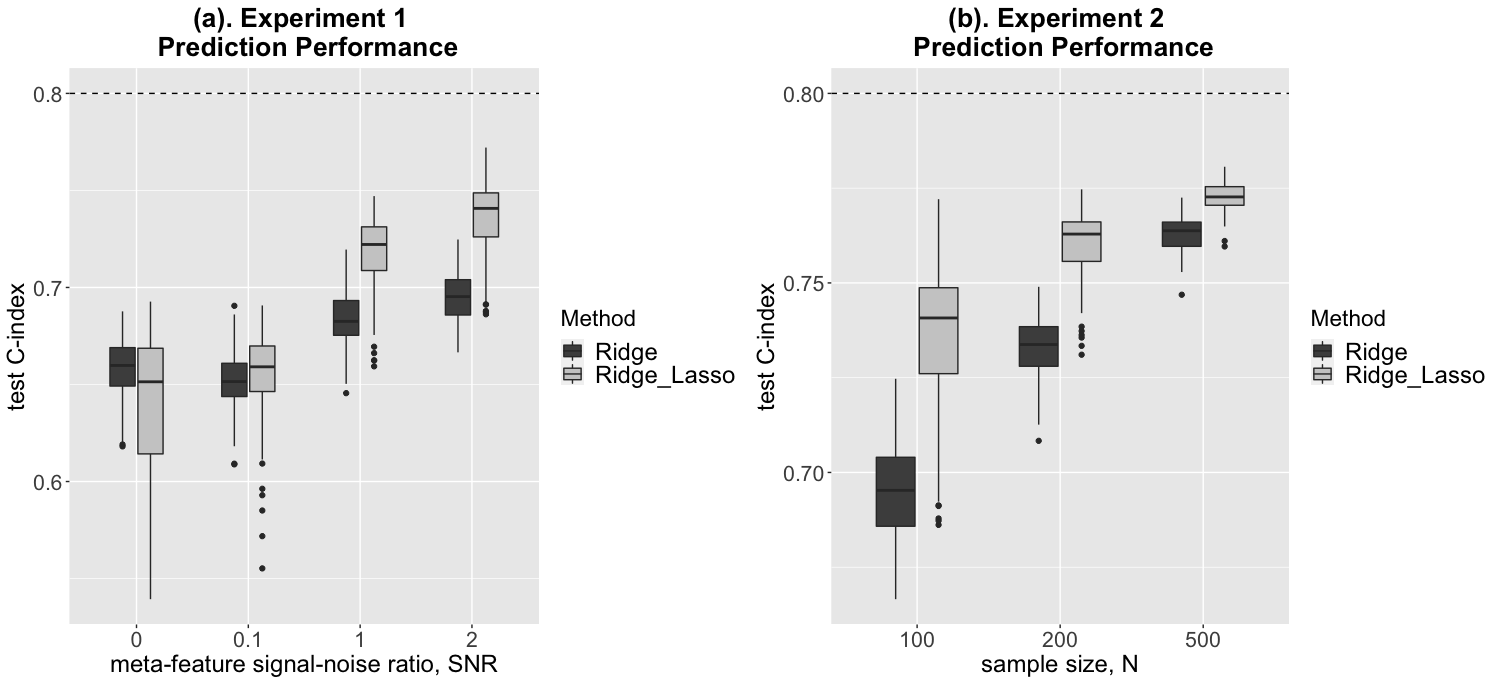
\includegraphics[width=\textwidth]{C12}
    \caption{Simulation: `xrnet' prediction performance (i)}
    \label{fig:C12}
\end{figure} 

\begin{figure}[H]
    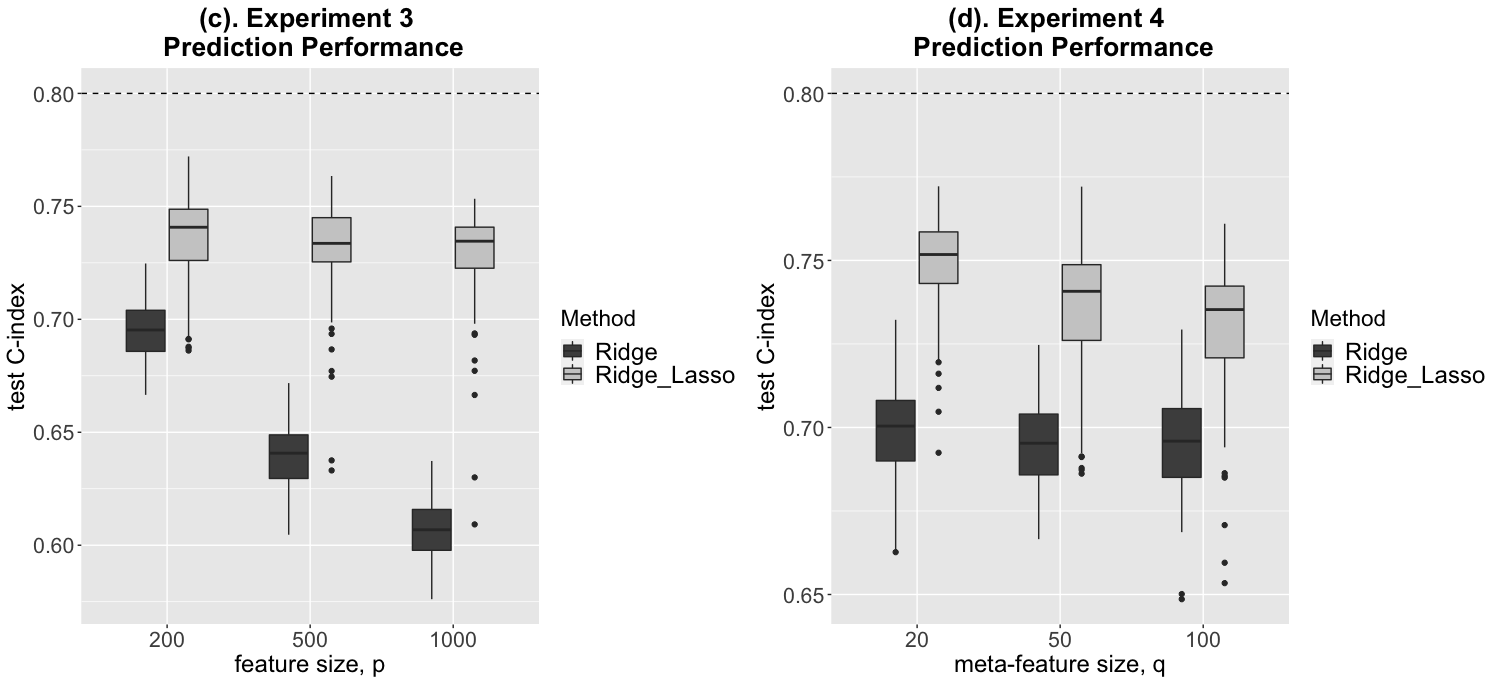
\includegraphics[width=\textwidth]{C34}
    \caption{Simulation: `xrnet' prediction performance (ii)}
    \label{fig:C34}
\end{figure} 

\begin{figure}[H]
    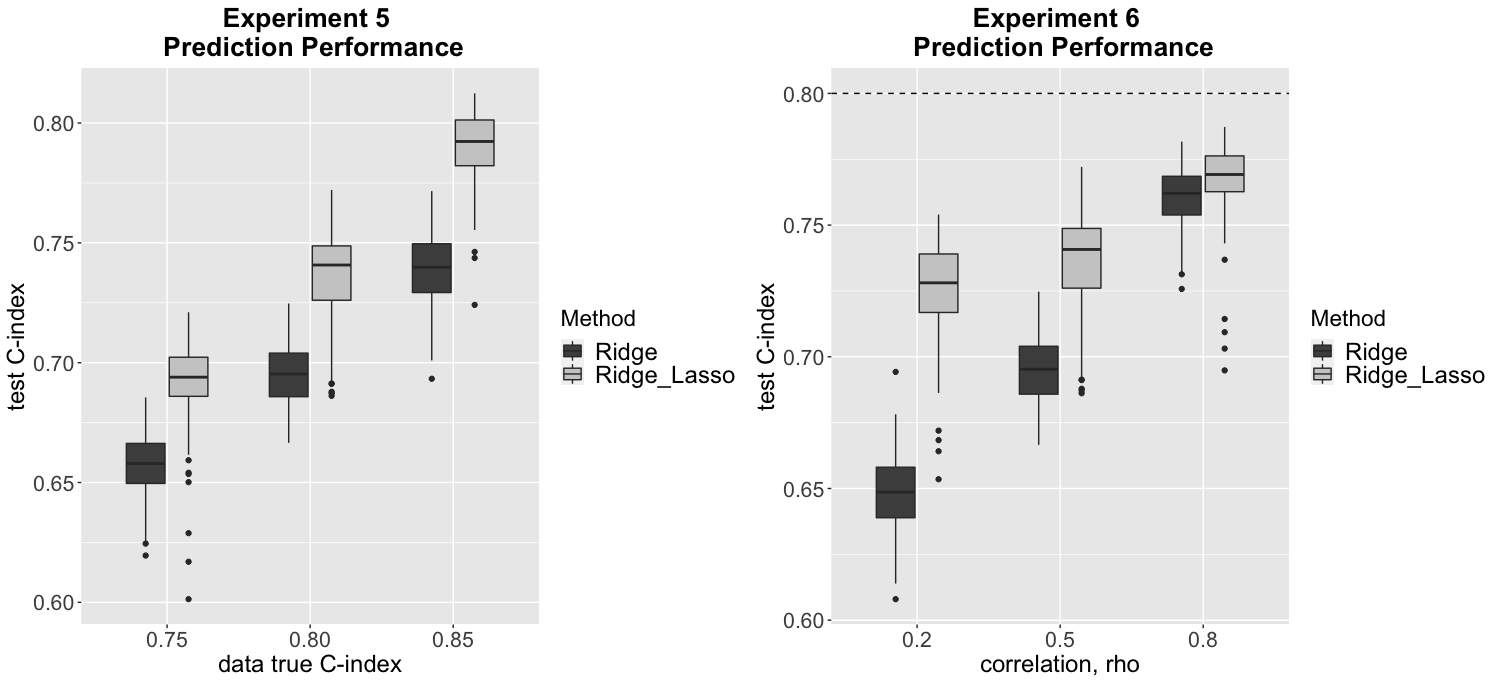
\includegraphics[width=\textwidth]{C56}
    \caption{Simulation: `xrnet' prediction performance (iii)}
    \label{fig:C56}
\end{figure} 

\begin{figure}[H]
    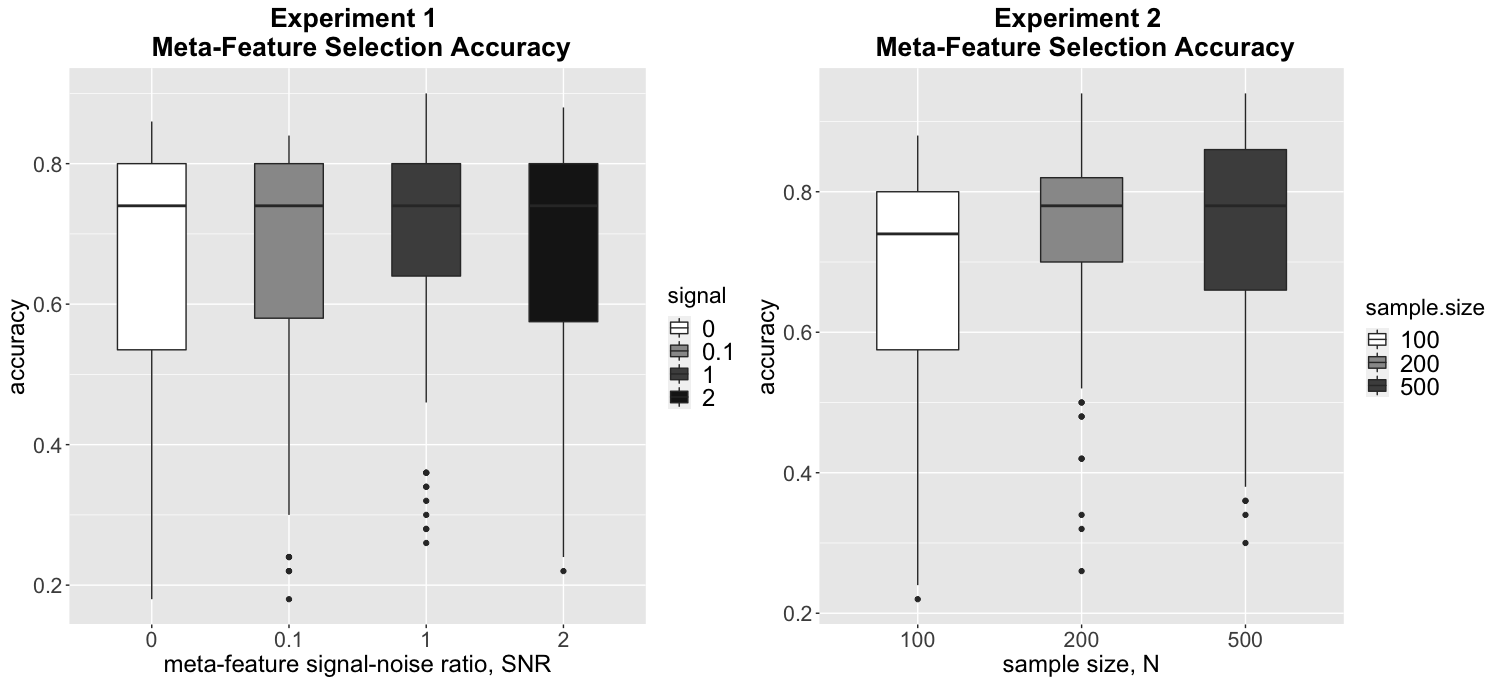
\includegraphics[width=\textwidth]{acc12}
    \caption{Simulation: `xrnet' meta-feature selection (i)}
    \label{fig:acc12}
\end{figure} 

\begin{figure}[H]
    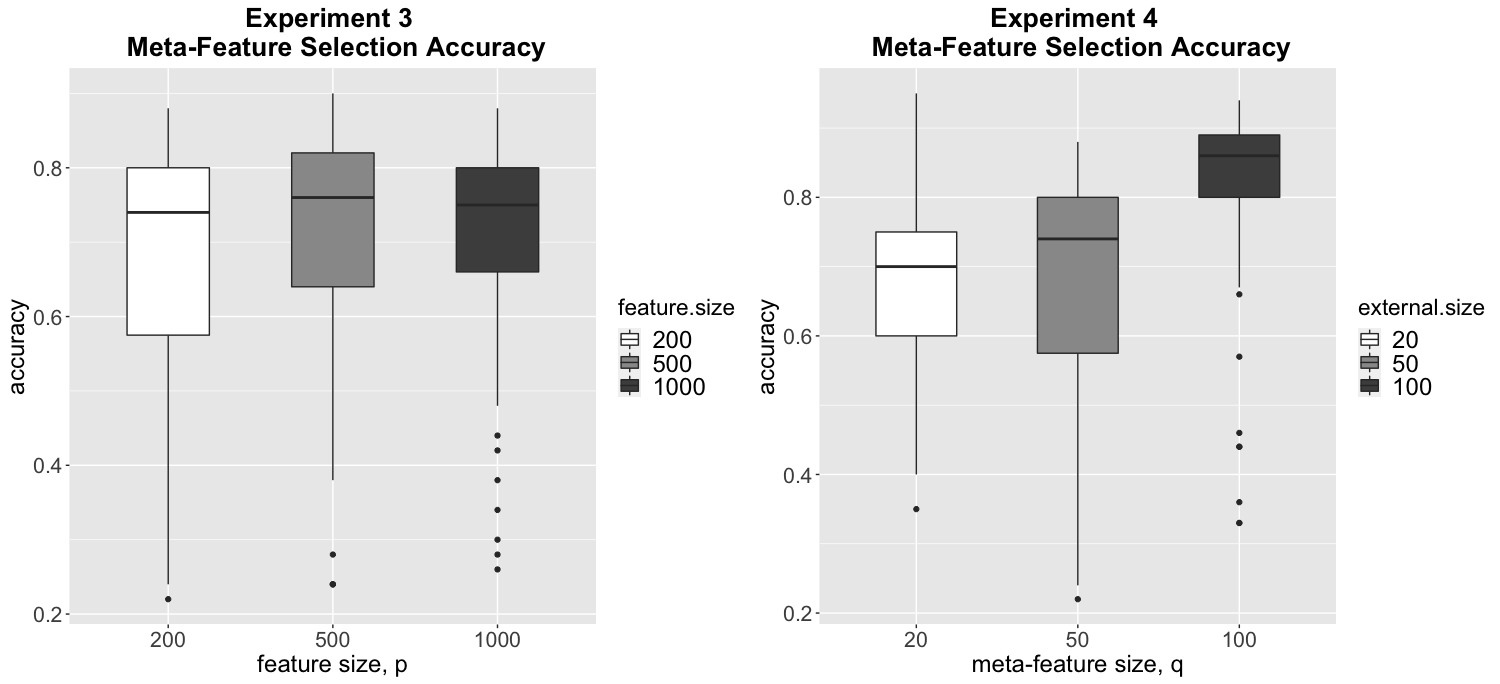
\includegraphics[width=\textwidth]{acc34}
    \caption{Simulation: `xrnet' meta-feature selection (ii)}
    \label{fig:acc34}
\end{figure} 

\begin{figure}[H]
    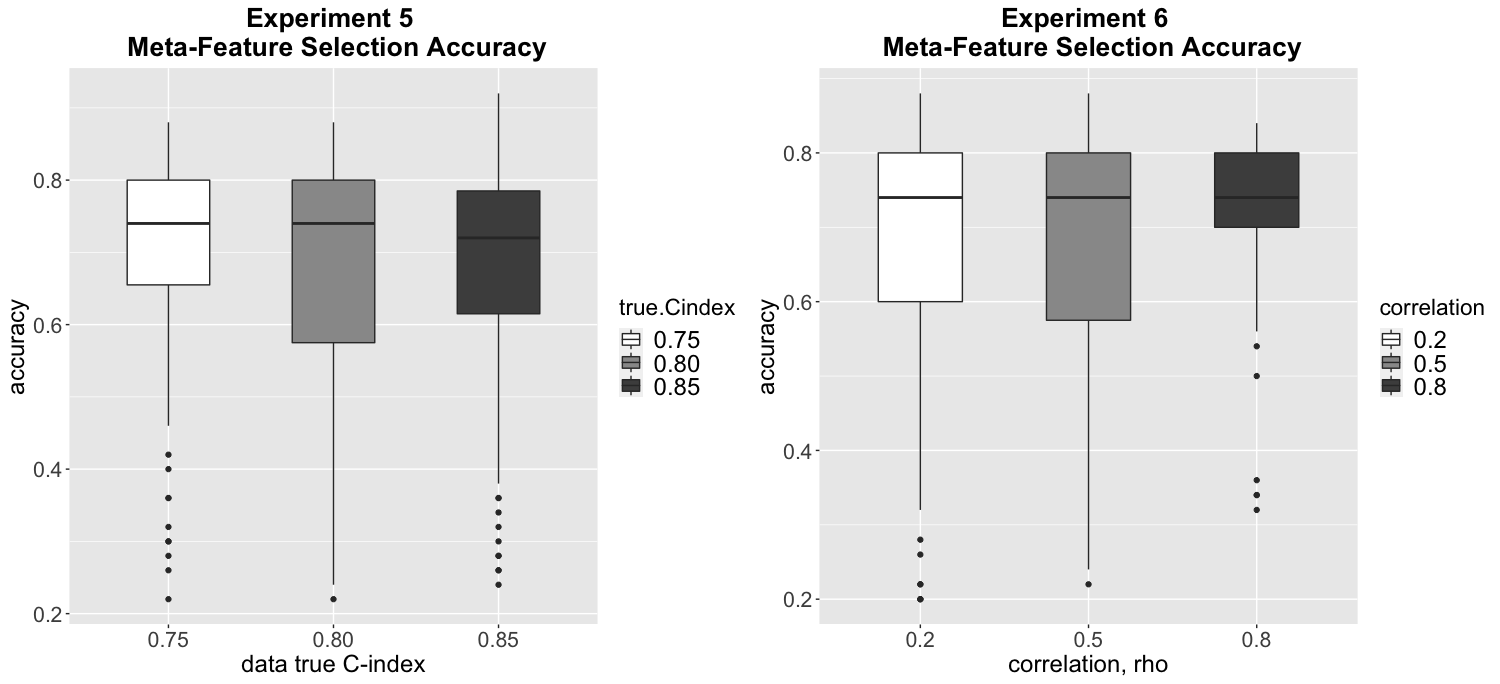
\includegraphics[width=\textwidth]{acc56}
    \caption{Simulation: `xrnet' meta-feature selection (iii)}
    \label{fig:acc56}
\end{figure} 

\section{Appendix for chapter 3}
\subsection{More simulation results}
We conducted 4 experiments for the meta-feature guided regularized regression model. The base case scenario is high meta-feature informativeness, sample size $N=100$, number of features $p=200$, number of meta-features $q=10$. In every experiment, we vary one of the 4 parameters and hold others fixed. We have seen the prediction performance results (Figure \ref{fig:sim21}), here we show feature selection accuracy, and number of features selected.

\begin{figure}[H]
    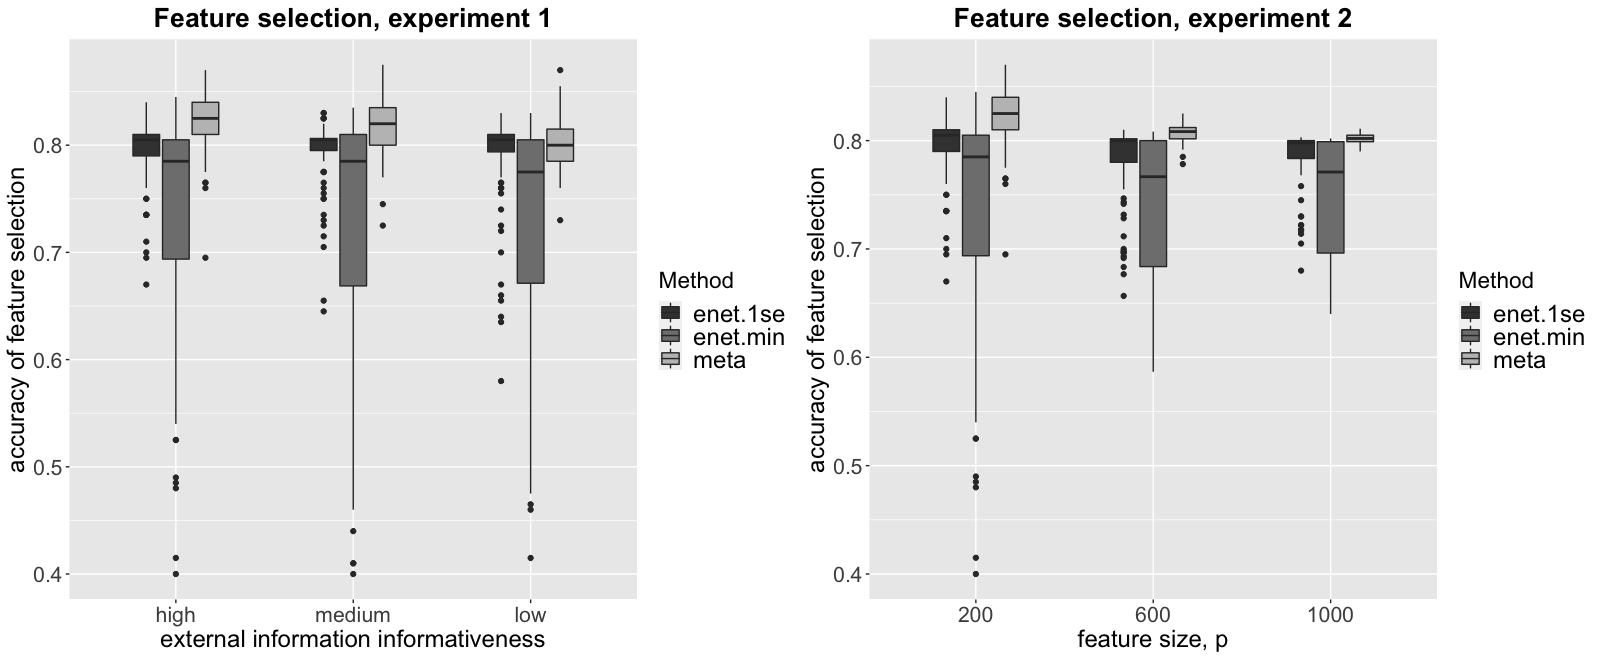
\includegraphics[width=\textwidth]{acc212}
    \caption{Simulation: meta guided feature selection accuracy (i)}
    \label{fig:acc212}
\end{figure} 

\begin{figure}[H]
    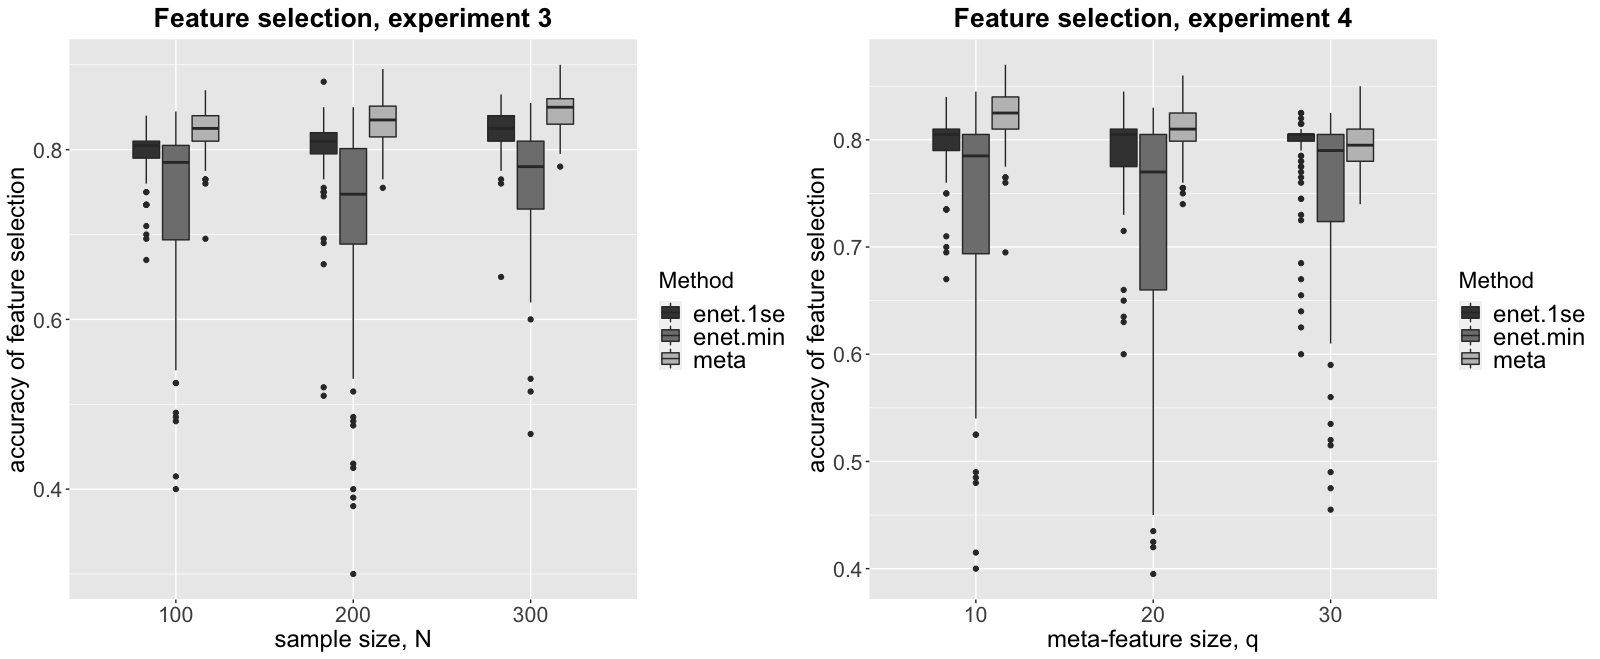
\includegraphics[width=\textwidth]{acc234}
    \caption{Simulation: meta guided feature selection accuracy (ii)}
    \label{fig:acc234}
\end{figure} 

\begin{figure}[H]
    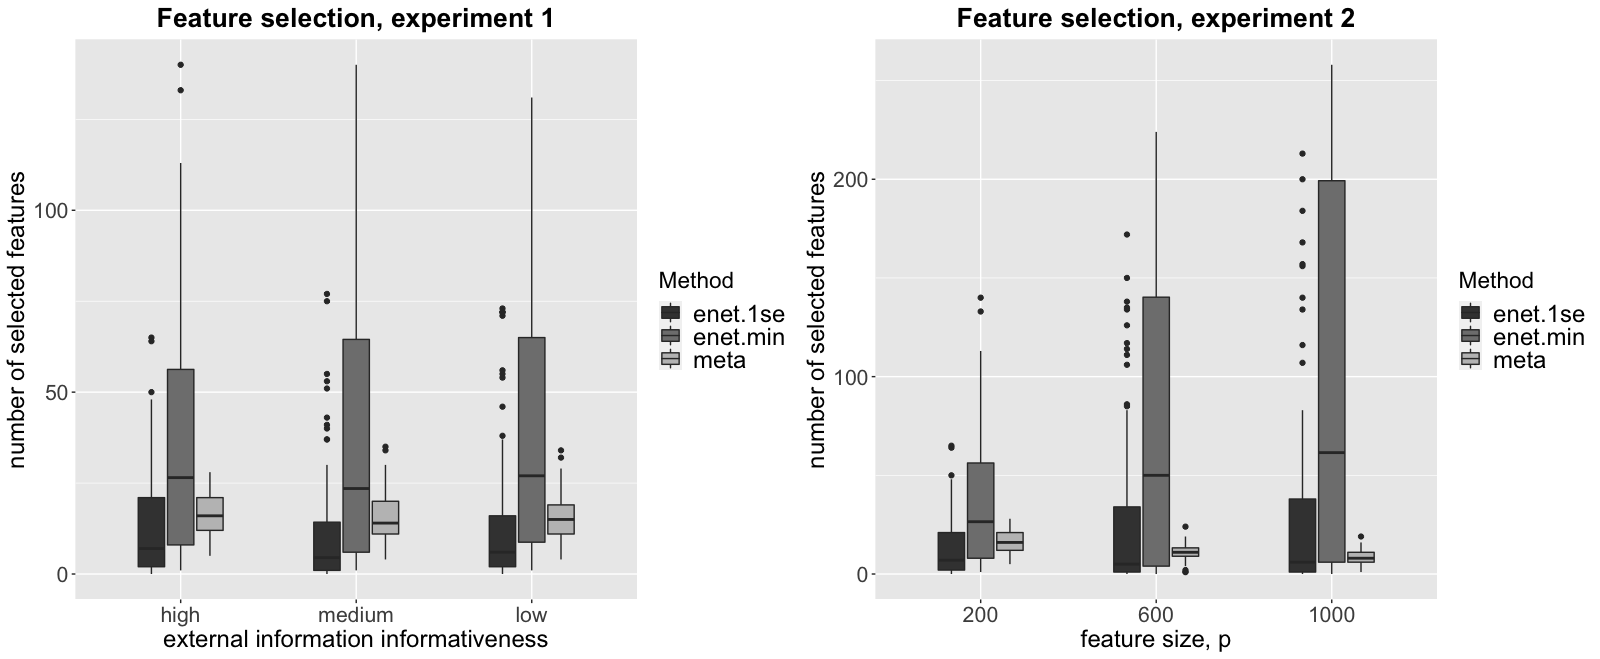
\includegraphics[width=\textwidth]{sel212}
    \caption{Simulation: meta guided number of selected features (i)}
    \label{fig:sel212}
\end{figure} 

\begin{figure}[H]
    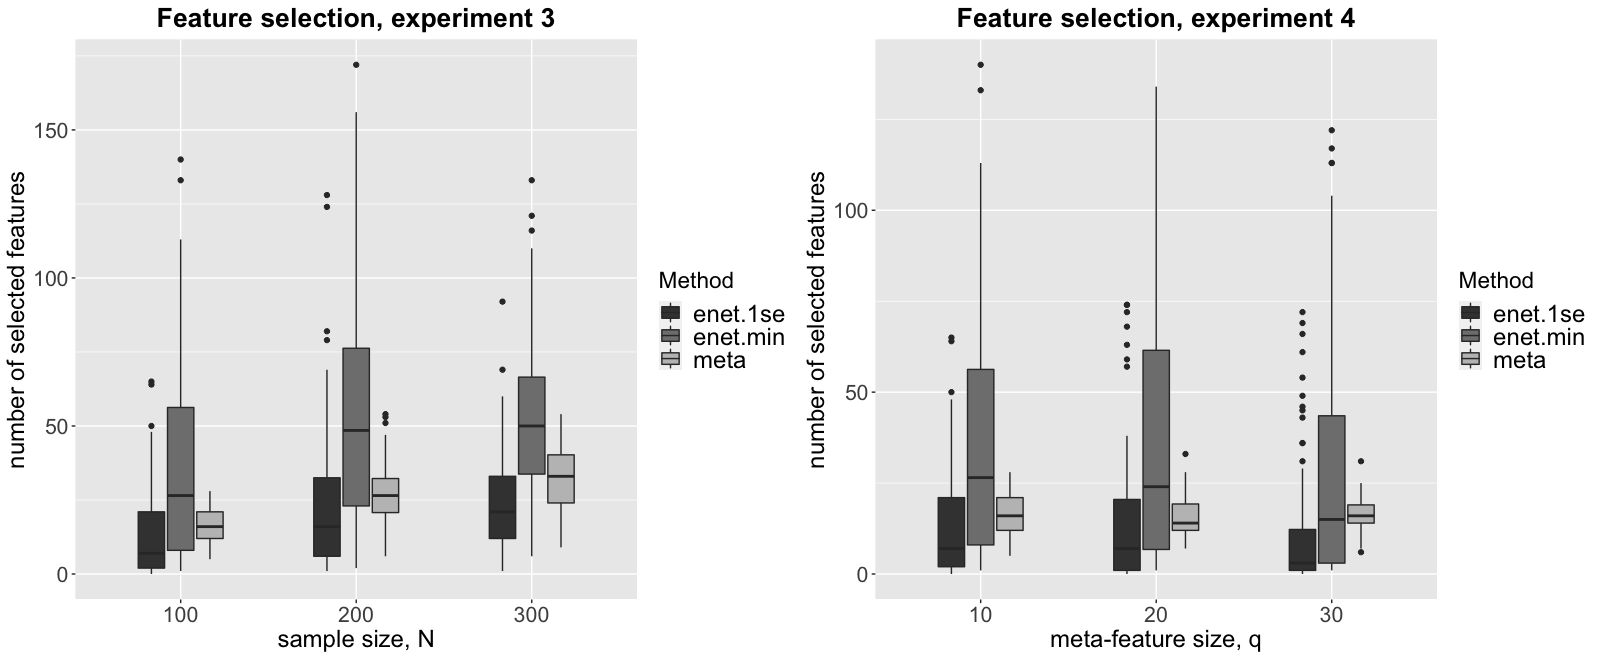
\includegraphics[width=\textwidth]{sel234}
    \caption{Simulation: meta guided number of selected features (ii)}
    \label{fig:sel234}
\end{figure} 

